\documentclass[book, b5paper, fittopage]{ncc}
\FromMargins[hf]{20mm}{20mm}{15mm}{15mm}

\usepackage[headings]{ncchdr}
\usepackage{graphicx}
\usepackage{charter}
\usepackage{booktabs}
\usepackage{multirow}
\usepackage{amssymb,amsmath}
\usepackage{ifxetex,ifluatex}

\usepackage[unicode=true]{hyperref}
\PassOptionsToPackage{hyphens}{url} % url is loaded by hyperref
\urlstyle{same}  % don't use monospace font for urls

\usepackage{parskip}
\setlength{\emergencystretch}{3em}  % prevent overfull lines

% set default figure placement to htbp
\makeatletter
\def\fps@figure{htbp}
\makeatother

% change verbatim and texttt style
\usepackage{fancyvrb,newverbs,xcolor}
\usepackage{letltxmacro}

\definecolor{cverbbg}{gray}{0.96}

\LetLtxMacro{\oldverbatim}{\verbatim}
\renewenvironment{verbatim}
 {\SaveVerbatim{cverb}}
 {\endSaveVerbatim
  % \center
  \flushleft\fboxrule=0pt
  \fboxsep=1em
  \colorbox{cverbbg}{\footnotesize\BUseVerbatim{cverb}}%
  \endflushleft
}

\LetLtxMacro{\oldtexttt}{\texttt}
\renewcommand{\texttt}[1]{\colorbox{cverbbg}{\oldtexttt{#1}}}



% ---------------------- start of content ----------------------------

\title{
  The 1090MHz Riddle \\
  \medskip
  \large An open-access book about decoding Mode-S and ADS-B data
}
\date{}
\author{Junzi Sun}

\begin{document}
% \maketitle

\clearpage

%% temporary titles
% command to provide stretchy vertical space in proportion
\newcommand\nbvspace[1][3]{\vspace*{\stretch{#1}}}
% allow some slack to avoid under/overfull boxes
\newcommand\nbstretchyspace{\spaceskip0.5em plus 0.25em minus 0.25em}
% To improve spacing on titlepages
\newcommand{\nbtitlestretch}{\spaceskip0.6em}

\thispagestyle{empty}


\begin{center}
\bfseries
\nbvspace[1]
\Huge
{\nbtitlestretch\huge
The 1090MHz Riddle}

\nbvspace[1]
\large
An open-access book about decoding Mode-S and ADS-B data

\nbvspace[1]
\small BY\\
\Large Junzi Sun\\[0.5em]

\nbvspace[2]

% \includegraphics[width=1.5in]{./graphics/pic37}
\nbvspace[3]
\normalsize

% \large
% Published by mode-s.org

\nbvspace[1]

\normalsize
GNU GPL v2 open-source license.

\nbvspace[1]
\end{center}


\pagestyle{headings}
\chapter*{Preface}
% WHY THIS BOOK? WHY USEFUL? WHAT PURPOSE? 2/3 SENTENCES
% say this is second edition???

This book provides a practical guide to decoding ADS-B and other types of common Mode S messages. Firstly, it consolidates the information from various ICAO documentation to provide readers easy access to key knowledge of Mode S and ADS-B and related topics. Secondly, examples and sample Python code are used extensively in the book to explain the decoding process.

Back in 2015, I joined Delft University of Technology to undertake PhD research on analyzing and modeling aircraft performance using open aircraft surveillance data. ADS-B data served as my primary data source.

Frustrated with the lack of open literature on ADS-B and Mode S, I created a live online project to document my experience in decoding ADS-B data, the \emph{ADS-B Decoding Guide}. As the guide grew in popularity, I started to receive questions, feedback, suggestions from the research community all over the world. These inputs greatly helped me to fix and improve the content of the decoding guide.

At the same time, I also started to incorporate Mode S Enhanced Surveillance data into my research, which required me to further develop tools for inferring and decoding new types of messages. At the same time, I created more content for the \emph{ADS-B Decoding Guide}. Due to the increasing interest expressed and demand from readers, I started writing a more comprehensive book focused on the decoding practice of the data, which was the starting point of this book.

Alongside the book, I also created a Python library, pyModeS, which welcomed contributions from GitHub users from all over the world. The evolution of pyModeS proceeded more quickly than the updating of the book. 

In 2019, I completed my PhD and continued as a faculty member in the aerospace engineering faculty of TU Delft. By then, I had time to reflect on aircraft surveillance data from a new perspective and determined that much of the book content could be updated.

The result is this text, which is both the second edition of \emph{the 1090 Megahertz Riddle} and one of the first books published under the TU Delft's OPEN publishing initiative. The book is published as open access book, under the CC-BY-NC-SA 4.0 license. The \LaTeX~source of the book is also shared on GitHub, where comments and pull requests are greatly appreciated.

\vspace{1cm}

\begin{flushright}
  Junzi Sun \\
  Delft, the Netherlands \\
  18th of August, 2020
\end{flushright}


\tableofcontents


\chapter{ADS-B}

ADS-B is short for Automatic Dependent Surveillance–Broadcast. It is a satellite based surveillance system. Aircraft position, velocity, together with identification are transmitted through Mode-S Extended Squitter (1090 MHz).

Majority of the aircraft nowadays are broadcasting ADS-B messages constantly. There are many ways you can set up you own receiver and antenna to start tapping into those signals (DVB-T usb stick, ModeSBeast, Raspberry Pi, RadarScape, etc).


\section{ADS-B Basics}\label{introduction}

\subsection{Message structure}\label{message-structure}

An ADS-B message is 112 bits long, and consists of 5 parts.

\begin{verbatim}
+--------+--------+-----------+--------------------------+---------+
|  DF 5  |  ** 3  |  ICAO 24  |          DATA 56         |  PI 24  |
+--------+--------+-----------+--------------------------+---------+
\end{verbatim}

Any ADS-B must start with the Downlink Format 17, or 18 in case of TIS-B message. They correspond to 10001 or 10010 in binary for the first 5 bits. Bits 6-8 are used as an additional identifier, which has different meanings within each ADS-B subtype.

In following Table \ref{tb:adsb-structure}, the key information of a ADS-B message is listed.

\begin{table}[!ht]
\centering
\caption{Structure of ADS-B messages}
\label{tb:adsb-structure}
\begin{tabular}{@{}llll@{}}
\toprule
nBits & Bits & Abbr. & Name \\ \midrule
5 & 1 - 5 & DF & Downlink Format \\
3 & 6 - 8 & CA & Capability (additional identifier) \\
24 & 9 - 32 & ICAO & ICAO aircraft address \\
56 & 33 - 88 & DATA & Data \\
 & {[}33 - 37{]} & {[}TC{]} & Type code \\
24 & 89 - 112 & PI & Parity/Interrogator ID \\ \bottomrule
\end{tabular}
\end{table}

It is worth noting that the ADS-B Extended Squitter sent from a Mode S transponder use Downlink Format 17 (\texttt{DF=17}). Non-Transponder-Based ADS-B Transmitting Subsystems and TIS-B Transmitting equipment use Downlink Format 18 (\texttt{DF=18}). By using \texttt{DF=18} instead of \texttt{DF=17}, an ADS-B/TIS-B Receiving Subsystem will know that the message comes from equipment that cannot be interrogated.

An example:

\begin{verbatim}
Raw message in hexadecimal:
8D4840D6202CC371C32CE0576098

[00100]0000010110011
00001101110001110000
110010110011100000

-----+------------+--------------+----------------------+--------------
HEX  | 8D         | 4840D6       | 202CC371C32CE0       | 576098
-----+------------+--------------+----------------------+--------------
BIN  | 10001  101 | 010010000100 | [00100]0000010110011 | 010101110110
     |            | 000011010110 | 00001101110001110000 | 000010011000
     |            |              | 110010110011100000   |
-----+------------+--------------+----------------------+--------------
DEC  |  17    5   |              | [4] ...............  |
-----+------------+--------------+----------------------+--------------
     |  DF    CA  |   ICAO       | [TC] --- DATA -----  | PI
-----+------------+--------------+----------------------+--------------
\end{verbatim}

\subsection{ICAO address}\label{icao-address}

In each ADS-B message, the sender (originating aircraft) can be identified using the ICAO address. It is located from 9 to 32 bits in binary (or 3 to 8 in hexadecimal). In the example above, it is \texttt{4840D6} or \texttt{010010000100}.

An unique ICAO address is assigned to each Mode-S transponder of an aircraft. Thus this is a unique identifier for each aircraft. You can use the query tool (\href{https://junzis.com/adb/}{World Aircraft Database}) from mode-s.org to find out more about the aircraft with a given ICAO address. For instance, using the previous ICAO \texttt{4840D6} example, it will return the result of a \texttt{Fokker\ 70} with registration of \texttt{PH-KZD}.

In addition, you can download the database from the aforementioned website in CSV format.

\subsection{ADS-B message types}\label{ads-b-message-types}

To identify what information is contained in an ADS-B message, we need to take a look at the \texttt{Type\ Code} of the message, indicated at bits 33 - 37 of the ADS-B message (or first 5 bits of the \texttt{DATA} segment).

In following Table \ref{tb:adsb-tc}, the relationships between each \texttt{Type\ Code} and its information contained in the \texttt{DATA} segment are shown.

\begin{table}[!ht]
\centering
\caption{ADS-B Type Code and content}
\label{tb:adsb-tc}
\begin{tabular}{@{}ll@{}}
\toprule
Type Code & Content                              \\ \midrule
1 - 4     & Aircraft identification              \\
5 - 8     & Surface position                     \\
9 - 18    & Airborne position (w/ Baro Altitude) \\
19        & Airborne velocities                  \\
20 - 22   & Airborne position (w/ GNSS Height)   \\
23 - 27   & Reserved                             \\
28        & Aircraft status                      \\
29        & Target state and status information  \\
31        & Aircraft operation status            \\ \bottomrule
\end{tabular}
\end{table}

\subsection{ADS-B Checksum}\label{ads-b-checksum}

ADS-B uses a cyclic redundancy check to validate the correctness of the received message, where the last 24 bits are the parity bits. The following pseudo-code describes the CRC process:

\begin{verbatim}
GENERATOR = 1111111111111010000001001

MSG = binary("8D4840D6202CC371C32CE0576098")  # total 112 bits

FOR i FROM 0 TO 88:                           # 112 - 24 parity bits
  if MSG[i] is 1:
    MSG[i:i+24] = MSG[i:i+24] ^ GENERATOR

CRC = MSG[-24:]                               # last 24 bits

IF CRC not 0:
  MSG is corrupted

\end{verbatim}

For the implementation of CRC encoder in Python, refer to the pyModeS library function: \texttt{pyModeS.crc()}

A comprehensive documentation on Mode-S parity coding can be found:

\begin{verbatim}
Gertz, Jeffrey L. Fundamentals of mode s parity coding. No. ATC-117.
MASSACHUSETTS INST OF TECH LEXINGTON LINCOLN LAB, 1984. APA
\end{verbatim}

\section{Aircraft Identification}\label{aircraft-identification}

An aircraft identification message has \texttt{DF:\ 17\ or\ 18}, and \texttt{TC:\ 1\ to\ 4}, the 56-bit \texttt{DATA} field is configured as follows:

\begin{verbatim}
+------+------+------+------+------+------+------+------+------+------+
| TC,5 | EC,3 | C1,6 | C2,6 | C3,6 | C4,6 | C5,6 | C6,6 | C7,6 | C8,6 |
+------+------+------+------+------+------+------+------+------+------+

TC: Type code
EC: Emitter category
C*: A character
\end{verbatim}

To decode characters, a lookup table is needed for mapping numbers to characters. It is defined as follows, where the \texttt{\#} is not used, and \texttt{\_} represents a separation.

\begin{verbatim}
#ABCDEFGHIJKLMNOPQRSTUVWXYZ#####_###############0123456789######
\end{verbatim}

In summary, characters and their decimal representations are:

\begin{verbatim}
A - Z :   1 - 26
0 - 9 :  48 - 57
    _ :  32
\end{verbatim}

The \texttt{EC} value in combination with \texttt{TC} value defines the category of the aircraft (such as: heavy, large, small, light, glider, etc.). When \texttt{EC} is set to zeros, such information is not available.

For example:

\begin{verbatim}
8D4840D6202CC371C32CE0576098
\end{verbatim}

The structure of the message is as follows:

\begin{verbatim}
     DF... CA.  ICAO..  DATA..................  PI....
HEX: 8   D      4840D6  2   0     2CC371C32CE0  576098
BIN: 10001 101  ******  00100 000 ************  ******
DEC: 17    4            4     0
                        TC    *
\end{verbatim}


Note that \texttt{Type\ Code} is inside of the DATA frame (first 5 bits). With \texttt{DF=17} and \texttt{TC=4}, we can confirm this is an aircraft identification message. Aircraft \texttt{callsign} then can be decoded.

In the previous example message, it is easy to decode the \texttt{Data} segment:

\begin{verbatim}
HEX: 20         2CC371C32CE0
BIN: 00100000 | 001011 001100 001101 110001 110000 110010 110011 100000
DEC:          |   11     12     13     49     48     50     51     32
LTR:          |   K      L      M      1      0      2      3      _
\end{verbatim}

So the final aircraft callsign decoded is: \texttt{KLM1023}

For detailed codes in Python, refer to the pyModeS library function: \texttt{pyModeS.adsb.callsign()}

\section{Compact Position Reporting}\label{compact-position-reporting}

The position information in ADS-B messages is encoded in a compact position reporting (CPR) format. The general idea behind CPR is to be able to encode more coordinate decimals using less bits. It is achieved by trading global position ambiguity and time with local position accuracy.

\subsection{Example}\label{example}

An easy example to understand the principle behind CPR:

Imaging the world is constructed by 16 grid, which we have divided into two levels, each level is encoded with two bits. Higher levels in color are \texttt{00} (yellow), \texttt{01} (blue), \texttt{10} (red), \texttt{11} (green). And within each color grid, the lower levels are also encoded similarly.

Then each grid can be represented as 4 digits from \texttt{0000} to \texttt{1111}. Now, we want to describe the movement indicated as the arrows in the green grids \texttt{1100\ -\textgreater{}\ 1101}, but we only have 3 bits to encode each position.

\begin{figure}
  \center
  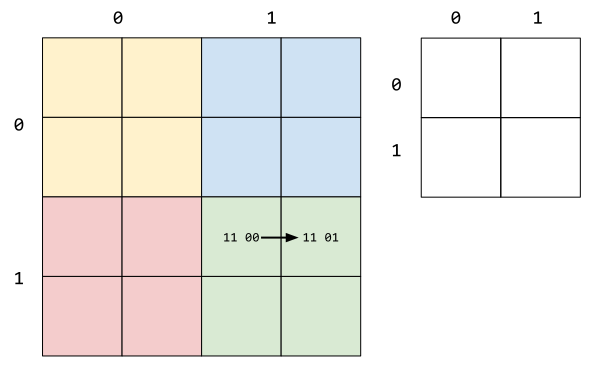
\includegraphics[width=8cm]{images/illustration-cpr-1.pdf}
\end{figure}

It is easy to see that the high 2 bits appeared in all positions, so we can define a structure to do the following:

\begin{enumerate}
  \item The last two bits shall represent the local position
  \item The combination of first digit from two messages defines the higher grid
\end{enumerate}

Then the two messages can be sent as \texttt{1\ 00\ -\textgreater{}\ 1\ 01}.

From lower bits \texttt{00\ -\textgreater{}\ 01}, we have four different possibility of movement as shown in dashed arrows, and from the two first bits combination \texttt{11}, we know that the arrow shall represent the movement in the green grids:

\begin{figure}
  \center
  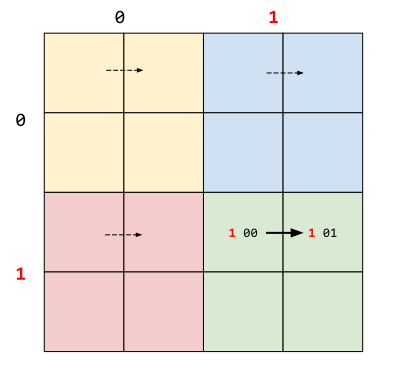
\includegraphics[width=5.5cm]{images/illustration-cpr-2.pdf}
\end{figure}

\subsection{The CPR and functions}\label{the-cpr-and-functions}

The actual CPR algorithm of course is more complicated, but the principle is very similar to the previous example. If only one message is given, it is possible to find multiple solutions that are spaced around the world. The combination of two (different types of) messages will yield the final result.

In CPR encoding, the Earth is divided in many zones (similar to the grid in the previous example). And the encoding algorithm is also more complicated (described in a later section). First, we will list some of the parameters and common functions used in the decoding process here.

\subsubsection{NZ}\label{nz}

Number of geographic latitude zones between equator and a pole. It is set to \texttt{NZ\ =\ 15} for Mode-S CPR encoding.

\subsubsection{floor(x)}\label{floorx}

the floor function \texttt{floor(x)} defines as the greatest integer value k, such that \texttt{k\textless{}=x}, for example:

\begin{verbatim}
floor(5.6) = 5
floor(-5.6) = -6
\end{verbatim}

\subsubsection{mod(x, y)}\label{modx-y}

the modulus function \texttt{mod(x,\ y)} returns:

\begin{equation}
  x - y \cdot floor(\frac{x}{y})
\end{equation}

where \texttt{y} can not be zero

\subsubsection{NL(lat)}\label{nllat}

Denotes the ``number of longitude zones'' function, given the latitude angle \texttt{lat}. The returned integer value is constrained within \texttt{{[}1,\ 59{]}}, calculated as:

\begin{equation}
  \text{NL}(lat) = floor \left( \frac{2 \pi}{\arccos(1 - \frac{1-\cos(\frac{\pi}{2 \cdot \text{NZ}})}{\cos^2(\frac{\pi}{180} \cdot \text{lat})}) } \right)
\end{equation}

For latitudes that are close to the equator or the poles, one of following values is returned:

\begin{verbatim}
lat = 0     ->    NL = 59
lat = +87   ->    NL = 2
lat = -87   ->    NL = 2
lat > +87   ->    NL = 1
lat < -87   ->    NL = 1
\end{verbatim}

\section{Airborne Positions}\label{airborne-positions}

An aircraft airborne position message has downlink format \texttt{17} (or \texttt{18}) with type code from \texttt{9} to \texttt{18}

Messages are composed as shown in following Table \ref{tb:adsb-pos-bits}

\begin{table}[!ht]
\centering
\caption{Airborne position message bits explained}
\label{tb:adsb-pos-bits}
\begin{tabular}{@{}llll@{}}
\toprule
Data Bits & MSG Bits & N-bit & Abbr    & Content                 \\ \midrule
33 - 37   & 1 - 5    & 5     & TC      & Type code               \\
38 - 39   & 6 - 7    & 2     & SS      & Surveillance status     \\
40        & 8        & 1     & NICsb   & NIC supplement-B        \\
41 - 52   & 9 - 20   & 12    & ALT     & Altitude                \\
53        & 21       & 1     & T       & Time                    \\
54        & 22       & 1     & F       & CPR odd/even frame flag \\
55 - 71   & 23 - 39  & 17    & LAT-CPR & Latitude in CPR format  \\
72 - 88   & 40 - 56  & 17    & LON-CPR & Longitude in CPR format \\ \bottomrule
\end{tabular}
\end{table}

Two types of the position messages (odd and even frames) are broadcast alternately. There are two different ways to decode an airborne position base on these messages:

\begin{enumerate}
\def\labelenumi{\arabic{enumi}.}

\item
  Unknown position, using both type of messages (aka globally unambiguous position)
\item
  Knowing previous position, using only one message (aka locally unambiguous position)
\end{enumerate}

Note: The definition of functions \texttt{NL(lat)}, \texttt{floor(x)}, and \texttt{mod(x,y)} are described in the CPR chapter.

\subsection{Globally unambiguous position (decoding with two messages)}\label{globally-unambiguous-position-decoding-with-two-messages}

\subsubsection{odd or even message?}\label{odd-or-even-message}

For each frame, bit 54 determines whether it is an odd or even frame:

\begin{verbatim}
0 -> Even frame
1 -> Odd frame
\end{verbatim}

For example, the two following messages are received:

\begin{verbatim}
8D40621D58C382D690C8AC2863A7
8D40621D58C386435CC412692AD6

|    | ICAO24 |      DATA      |  CRC   |
|----|--------|----------------|--------|
| 8D | 40621D | 58C382D690C8AC | 2863A7 |
| 8D | 40621D | 58C386435CC412 | 692AD6 |

\end{verbatim}

The payload data in binary formation:

\begin{verbatim}
| DATA                                                                       |
|============================================================================|
| TC    | ... | ALT          | T | F | CPR-LAT           | CPR-LON           |
|-------|-----|--------------|---|---|-------------------|-------------------|
| 01011 | 000 | 110000111000 | 0 | 0 | 10110101101001000 | 01100100010101100 |
| 01011 | 000 | 110000111000 | 0 | 1 | 10010000110101110 | 01100010000010010 |
\end{verbatim}

In both messages we can find \texttt{DF=17} and \texttt{TC=11}, with the same ICAO24 address \texttt{40621D}. So, those two frames are valid for decoding the positions of this aircraft. Assume the first message is the newest message received.

\subsubsection{The CPR representation of
coordinates}\label{the-cpr-representation-of-coordinates}

\begin{verbatim}
| F | CPR Latitude      | CPR Longitude     |
|---|-------------------|-------------------|
| 0 | 10110101101001000 | 01100100010101100 |  -> newest
| 1 | 10010000110101110 | 01100010000010010 |
|---|-------------------|-------------------|

In decimal:

|---|-------------------|-------------------|
| 0 | 93000             | 51372             |
| 1 | 74158             | 50194             |
|---|-------------------|-------------------|

CPR_LAT_EVEN: 93000 / 131072 -> 0.7095
CPR_LON_EVEN: 51372 / 131072 -> 0.3919
CPR_LAT_ODD:  74158 / 131072 -> 0.5658
CPR_LON_ODD:  50194 / 131072 -> 0.3829
\end{verbatim}

Since CPR latitude and longitude are encoded in 17 bits, 131072 ($2^17$) is the maximum value.

\subsubsection{Calculate the latitude index j}\label{calculate-the-latitude-index-j}

Use the following equation:

\begin{equation}
  j = floor \left( 59 \cdot \mathrm{Lat}_\mathrm{cprEven} - 60 \cdot \mathrm{Lat}_\mathrm{cprOdd} + \frac{1}{2}  \right)
\end{equation}

\noindent where $j$ is set 8.

\subsubsection{Calculate latitude}\label{calculate-latitude}

First, two constants will be used:

\begin{equation}
  \begin{split}
    \mathrm{dLat}_\mathrm{even} &= \frac{360}{4 \cdot NZ} = \frac{360}{60} \\
    \mathrm{dLat}_\mathrm{odd} &= \frac{360}{4 \cdot NZ - 1}  = \frac{360}{59}
  \end{split}
\end{equation}

Then we can use the following equations to compute the relative latitudes:

\begin{equation}
  \begin{split}
    \mathrm{Lat}_\mathrm{even} &= \mathrm{dLat}_\mathrm{even} \cdot [mod(j, 60) + \mathrm{Lat}_\mathrm{cprEven}] \\
    \mathrm{Lat}_\mathrm{odd} &= \mathrm{dLat}_\mathrm{odd} \cdot [mod(j, 59) + \mathrm{Lat}_\mathrm{cprOdd}]
  \end{split}
\end{equation}

For the southern hemisphere, values will fall from 270 to 360 degrees. We need to make sure the latitude is within the range
\texttt{{[}-90,\ +90{]}}:

\begin{equation}
  \begin{split}
    \mathrm{Lat}_\mathrm{even} &= \mathrm{Lat}_\mathrm{even} - 360  \quad \text{if } (\mathrm{Lat}_\mathrm{even} \geq 270) \\
    \mathrm{Lat}_\mathrm{odd} &= \mathrm{Lat}_\mathrm{odd} - 360  \quad \text{if } (\mathrm{Lat}_\mathrm{odd} \geq 270)
  \end{split}
\end{equation}

Final latitude is chosen depending on the time stamp of the frames, the newest one, is used:

\begin{equation}
  \mathrm{Lat} =
  \begin{cases}
   \mathrm{Lat}_\mathrm{even}     & \text{if } (T_\mathrm{even} \geq T_\mathrm{odd}) \\
   \mathrm{Lat}_\mathrm{odd}     & \text{else}
  \end{cases}
\end{equation}

In the example:

\begin{verbatim}
Lat_EVEN = 52.25720214843750
Lat_ODD  = 52.26578017412606
Lat = Lat_EVEN = 52.25720
\end{verbatim}

\subsubsection{Check the latitude zone
consistency}\label{check-the-latitude-zone-consistency}

Compute \texttt{NL(Lat\_E)} and \texttt{NL(Lat\_O)}. If not the same, two positions are located at different latitude zones. Computation of a global longitude is not possible. Exit the calculation and wait for new messages. If two values are the same, we proceed to longitude calculation.

\subsubsection{Calculate longitude}\label{calculate-longitude}

If the even frame comes latest \texttt{T\_EVEN\ \textgreater{}\ T\_ODD}:

\begin{equation}
  \begin{split}
    ni &= max \left( NL(\mathrm{Lat}_\mathrm{even}), 1 \right) \\
    \mathrm{dLon} &= \frac{360}{ni} \\
    m &= floor \left\{ Lon_\mathrm{cprEven} \cdot [NL(\mathrm{Lat}_\mathrm{even})-1] - Lon_\mathrm{cprOdd} \cdot NL(\mathrm{Lat}_\mathrm{even}) + \frac{1}{2}  \right\} \\
    \mathrm{Lon} &= \mathrm{dLon} \cdot \left( mod(m, ni) + Lon_\mathrm{cprEven} \right)
  \end{split}
\end{equation}

In case where the odd frame comes latest
\texttt{T\_EVEN\ \textless{}\ T\_ODD}:

\begin{equation}
  \begin{split}
    ni &= max \left( NL(\mathrm{Lat}_\mathrm{odd})-1, 1 \right) \\
    \mathrm{dLon} &= \frac{360}{ni} \\
    m &= floor \left\{ Lon_\mathrm{cprEven} \cdot [NL(\mathrm{Lat}_\mathrm{odd})-1] - Lon_\mathrm{cprOdd} \cdot NL(\mathrm{Lat}_\mathrm{odd}) + \frac{1}{2}  \right\} \\
    \mathrm{Lon} &= \mathrm{dLon} \cdot \left( mod(m, ni) + Lon_\mathrm{cprOdd} \right)
  \end{split}
\end{equation}

if the result is larger than 180 degrees:

\begin{equation}
  \mathrm{Lon} = \mathrm{Lon} - 360  \quad \text{if } (\mathrm{Lon} \geq 180)
\end{equation}

In the example:

\begin{verbatim}
Lon:  3.91937
\end{verbatim}

Here is a Python implementation:
\url{https://github.com/junzis/pyModeS/blob/faf4313/pyModeS/adsb.py\#L166}

\subsubsection{Calculate altitude}\label{calculate-altitude}

The altitude of the aircraft is much easier to compute from the data frame. The bits in the altitude field (either odd or even frame) are as follows:

\begin{verbatim}
1100001 1 1000
        ^
       Q-bit
\end{verbatim}

This Q-bit (bit 48) indicates whether the altitude is encoded in multiples of 25 or 100 ft (0: 100 ft, 1: 25 ft).

For Q = 1, we can calculate the altitude as follows:

First, remove the Q-bit :

\begin{verbatim}
N = 1100001 1000 => 1560 (in decimal)
\end{verbatim}

The final altitude value will be:

\begin{equation}
  Alt = N \cdot 25 - 1000 \quad \text{(ft.)}
\end{equation}

In this example, the altitude at which the aircraft is flying is:

\begin{verbatim}
1560 * 25 - 1000 = 38000 ft.
\end{verbatim}

Note that the altitude has the accuracy of +/- 25 ft when the Q-bit is 1, and the value can represent altitudes from -1000 to +50175 ft.

\subsubsection{The final position}\label{the-final-position}

Finally, we have all three components (latitude/longitude/altitude) of the aircraft position:

\begin{verbatim}
LAT: 52.25720 (degrees N)
LON:  3.91937 (degrees E)
ALT:    38000 ft
\end{verbatim}

\subsection{Locally unambiguous position (decoding with one
message)}\label{locally-unambiguous-position-decoding-with-one-message}

This method gives the possibility of decoding aircraft using only one message knowing a reference position. This method computes the latitude index (j) and the longitude index (m) based on such reference, and can be used with either type of the messages.

\subsubsection{The reference position}\label{the-reference-position}

The reference position should be close to the actual position (eg. position of aircraft previously decoded, or the location of ADS-B antenna), and must be \textbf{within a 180 NM} range.

\subsubsection{Calculate dLat}\label{calculate-dlat}

\begin{equation}
  dLat =
  \begin{cases}
   \frac{360}{4 \cdot NZ} = \frac{360}{60}          & \text{if even message}  \\
   \frac{360}{4 \cdot NZ - 1}  = \frac{360}{59}     & \text{if odd message}
  \end{cases}
\end{equation}

\subsubsection{Calculate the latitude indexj} \label{calculate-the-latitude-index-j-1}

\begin{equation}
  j = floor \left (\frac{\mathrm{Lat}_{ref}}{dLat} \right) + floor \left( \frac{mod(\mathrm{Lat}_{ref}, dLat)}{dLat}  - \mathrm{Lat}_\mathrm{cpr}  + \frac{1}{2} \right)
\end{equation}

\subsubsection{Calculate latitude}\label{calculate-latitude-1}

\begin{equation}
  \mathrm{Lat} = dLat \cdot (j + \mathrm{Lat}_\mathrm{cpr})
\end{equation}


\subsubsection{Calculate dLon}\label{calculate-dlon}

\begin{equation}
  \mathrm{dLon} =
  \begin{cases}
   \frac{360}{NL(Lat)}    & \text{if } NL(Lat) > 0  \\
   360                    & \text{if } NL(Lat) = 0
  \end{cases}
\end{equation}

\subsubsection{Calculate longitude index
m}\label{calculate-longitude-index-m}

\begin{equation}
  m = floor \left( \frac{Lon_{ref}}{\mathrm{dLon}} \right) + floor \left( \frac{mod(Lon_{ref}, \mathrm{dLon})}{\mathrm{dLon}}  - Lon_\mathrm{cpr}  + \frac{1}{2}  \right)
\end{equation}

\subsubsection{Calculate longitude}\label{calculate-longitude-1}

\begin{equation}
  Lon = \mathrm{dLon} \cdot (m + Lon_\mathrm{cpr})
\end{equation}

\subsubsection{Example}\label{example}

For the same example message:

\begin{verbatim}
8D40621D58C382D690C8AC2863A7

Reference position:
  LAT: 52.258
  LON:  3.918
\end{verbatim}

The structure of the message is:

\begin{verbatim}
8D40621D58C382D690C8AC2863A7

|    | ICAO24 |      DATA      |  CRC   |
|----|--------|----------------|--------|
| 8D | 40621D | 58C382D690C8AC | 2863A7 |


Data in binary:

| DATA                                                                       |
|============================================================================|
| TC    | ... | ALT          | T | F | CPR-LAT           | CPR-LON           |
|-------|-----|--------------|---|---|-------------------|-------------------|
| 01011 | 000 | 110000111000 | 0 | 0 | 10110101101001000 | 01100100010101100 |


CPR representation:

| F | CPR Latitude      | CPR Longitude     |
|---|-------------------|-------------------|
| 0 | 10110101101001000 | 01100100010101100 |
|---|-------------------|-------------------|
|   | 93000 / 131072    | 51372 / 131072    |
|   | 0.7095            | 0.3919            |
|---|-------------------|-------------------|

d_lat:  6
j:      8
lat:    52.25720
m:      0
d_lon:  10
lon:    3.91937
\end{verbatim}

\section{Airborne Velocity}\label{airborne-velocity}

There are two different types of messages for velocities, determined by
3-bit subtype in the message. With subtype 1 and 2, surface velocity
(ground speed) is reported. And in subtype 3 and 4, aircraft airspeed is
reported.

Type 2 and 4 are for supersonic aircraft. So, before we have another
commercial supersonic aircraft flying around, you won't see any of those
types.

In real world, very few of subtype 3 messages are reported. In our
setup, we only received \textbf{0.3\%} of these message with regards to
subtype 1.

An aircraft velocity message has \texttt{DF:\ 17\ or\ 18},
\texttt{TC:\ 19}, and the subtype codes are represented in bits 38 to
40. Now, we can decode those messages.

\subsection{Subtype 1 (Ground Speed)}\label{subtype-1-ground-speed}

Subtype 1 (subsonic, ground speed), are broadcast when ground velocity
information is available. The aircraft velocity contains speed and
heading information. The speed and heading are also decomposed into
North-South, and East-West components.

For example, the following message is received:

\begin{verbatim}
Message: 8D485020994409940838175B284F

|    | ICAO24 |      DATA      |  CRC   |
|----|--------|----------------|--------|
| 8D | 485020 | 99440994083817 | 5B284F |

Convert DATA [99440994083817] into binary:

|-------|-----|----|--------|-----|------|------------|
|  TC   | ST  | IC | RESV_A | NAC | S-EW | V-EW       |
|-------|-----|----|--------|-----|------|------------|
| 10011 | 001 | 0  | 1      | 000 | 1    | 0000001001 |

|------|------------|-------|------|-----------|--------|-------|---------|
| S-NS | V-NS       | VrSrc | S-Vr | Vr        | RESV_B | S_Dif | Dif     |
|------|------------|-------|------|-----------|--------|-------|---------|
| 1    | 0010100000 | 0     | 1    | 000001110 | 00     | 0     | 0010111 |
\end{verbatim}

There are quite a few parameters in the velocity message. From left to
right, the number of bits indicates the contents in following Table \ref{tb:adsb-v-bits-st-1}

\begin{table}[!ht]
\centering
\caption{Airborne velocity message bits explained - Subtype 1}
\label{tb:adsb-v-bits-st-1}
\begin{tabular}{@{}lllll@{}}
\toprule
MSG Bits & Data Bits & Len & Abbr    & Content                    \\ \midrule
33 - 37  & 1 - 5     & 5   & TC      & Type code                  \\
38 - 40  & 6 - 8     & 3   & ST      & Subtype                    \\
41       & 9         & 1   & IC      & Intent change flag         \\
42       & 10        & 1   & RESV\_A & Reserved-A                 \\
43 - 45  & 11 - 13   & 3   & NAC     & Velocity uncertainty (NAC) \\
46       & 14        & 1   & S\_ew   & East-West velocity sign    \\
47 - 56  & 15 - 24   & 10  & V\_ew   & East-West velocity         \\
57       & 25        & 1   & S\_ns   & North-South velocity sign  \\
58 - 67  & 26 - 35   & 10  & V\_ns   & North-South velocity       \\
68       & 36        & 1   & VrSrc   & Vertical rate source       \\
69       & 37        & 1   & S\_vr   & Vertical rate sign         \\
70 - 78  & 38 - 46   & 9   & Vr      & Vertical rate              \\
79 - 80  & 47 - 48   & 2   & RESV\_B & Reserved-B                 \\
81       & 49        & 1   & S\_Dif  & Diff from baro alt, sign   \\
82 - 88  & 50 - 66   & 7   & Dif     & Diff from baro alt         \\ \bottomrule
\end{tabular}
\end{table}


\subsubsection{Horizontal Velocity}\label{horizontal-velocity}

For calculating the horizontal speed and heading we need four values,
East-West Velocity \texttt{V\_ew}, East-West Velocity Sign
\texttt{S\_ew}, North-South Velocity \texttt{V\_ns}, North-South
Velocity Sign \texttt{S\_ns}. And pay attention on the directions
(signs) in the calculation.

\begin{verbatim}
S_ns:
    1 -> flying North to South
    0 -> flying South to North
S_ew:
    1 -> flying East to West
    0 -> flying West to East
\end{verbatim}

The Speed (v) and heading (h) with unit knot and degree can be computed
as follows:

\[V_{we} =
\begin{cases}
 -1 \cdot (V_{ew} - 1)    & \text{if } s_{ew} = 1 \\
 V_{ew} - 1         & \text{if } s_{ew} = 0
\end{cases}\]

\[V_{sn} =
\begin{cases}
 -1 \cdot (V_{ns} - 1)    & \text{if } s_{ns} = 1 \\
 V_{ns} - 1         & \text{if } s_{ns} = 0
\end{cases}\]

\[v = \sqrt{V_{we}^{2} + V_{sn}^{2}}\]

\[h = arctan2 \left( V_{we}, V_{sn} \right) \cdot \frac{360}{2\pi}  \quad \text{(deg)}\]

In case of a negative value here, we will simply add 360 degrees.

\[h = h + 360  \quad (\text{if } h < 0)\]

So, now we have the speed and heading of our example:

\begin{verbatim}
V-EW: 0000001001 -> 9
S-EW: 1
V-NS: 0010100000 -> 160
S-NS: 1

V_{we} = - (9 - 1) = -8
V_{sn} = - (160 - 1) = -159

v = 159.20 (kt)
h = 182.88 (deg)
\end{verbatim}

\subsubsection{Vertical Rate}\label{vertical-rate}

The direction of vertical movement of aircraft can be read from
\texttt{S\_vr} field, in message bit-69:

\begin{verbatim}
0 -> UP
1 -> Down
\end{verbatim}

The actual vertical rate \texttt{Vr} is the value of bits 70-78, minus
1, and then multiplied by 64 in \textbf{feet/minute} (ft/min). In our
example:

\begin{verbatim}
Vr-bits: 000001110 = 14
Vr: (14 - 1) x 64 => 832 fpm
S-Vr: 0 => Down / Descending
\end{verbatim}

So we see a descending aircraft at 832 ft/min rate of descend.

The Vertical Rate Source (VrSrc) field determines if it is a measurement
in barometric pressure altitude or geometric altitude:

\begin{verbatim}
0 ->  Baro-pressure altitude change rate
1 ->  Geometric altitude change rate
\end{verbatim}

\subsection{Subtype 3 (Airspeed)}\label{subtype-3-airspeed}

Subtype 3 (subsonic, airspeed), are broadcast when ground speed
information is NOT available, while airspeed is available. The structure
of the message is similar to the previous one. Let's take a close look
at an example for decoding here.

\begin{verbatim}
Message: 8DA05F219B06B6AF189400CBC33F

|    | ICAO24 |      DATA      |  CRC   |
|----|--------|----------------|--------|
| 8D | A05F21 | 9B06B6AF189400 | CBC33F |

Convert DATA [9B06B6AF189400] into binary:

|-------|-----|----|--------|-----|------|------------|------|------------|
|  TC   | ST  | IC | RESV_A | NAC | S_hdg| Hdg        | AS-t | AS         |
|-------|-----|----|--------|-----|------|------------|------|------------|
| 10011 | 011 | 0  | 0      | 000 | 1    | 1010110110 | 1    | 0101111000 |

|-------|------|-----------|--------|-------|---------|
| VrSrc | S-Vr | Vr        | RESV_B | S_Dif | Dif     |
|-------|------|-----------|--------|-------|---------|
| 1     | 1    | 000100101 | 00     | 0     | 0000000 |
\end{verbatim}

The details on all data bits are described in following Table \ref{tb:adsb-v-bits-st-3}:

\begin{table}[]
\centering
\caption{Airborne velocity message bits explained - Subtype 3}
\label{tb:adsb-v-bits-st-3}
\begin{tabular}{@{}lllll@{}}
\toprule
MSG Bits   & DATA Bits   & Len & Abbr    & Content                        \\ \midrule
33 - 37    & 1 - 5       & 5   & TC      & Type code                      \\
38 - 40    & 6 - 8       & 3   & ST      & Subtype                        \\
41         & 9           & 1   & IC      & Intent change flag             \\
42         & 10          & 1   & RESV\_A & Reserved-A                     \\
43 - 45    & 11 - 13     & 3   & NAC     & Velocity uncertainty (NAC)     \\
46         & 14          & 1   & S\_hdg  & Heading status                 \\
47 - 56    & 15 - 24     & 10  & Hdg     & Heading (proportion)           \\
57         & 25          & 1   & AS-t    & Airspeed Type                  \\
58 - 67    & 26 - 35     & 10  & AS      & Airspeed                       \\
68         & 36          & 1   & VrSrc   & Vertical rate source           \\
69         & 37          & 1   & S\_vr   & Vertical rate sign             \\
70 - 78    & 38 - 46     & 9   & Vr      & Vertical rate                  \\
79 - 80    & 47 - 48     & 2   & RESV\_B & Reserved-B                     \\
81         & 49          & 1   & S\_Dif  & Difference from baro alt, sign \\
82 - 88    & 50 - 66     & 7   & Dif     & Difference from baro alt       \\ \bottomrule
\end{tabular}
\end{table}

\subsubsection{Heading}\label{heading}

\texttt{S\_hdg} makes the status of heading data:

\begin{verbatim}
0 -> heading data not available
1 -> heading data available
\end{verbatim}

10-bits \texttt{Hdg} is the represent the proportion of the degrees of a
full circle, i.e. 360 degrees. (Note: 0000000000 - 1111111111 represents
0 - 1023 )

\[heading = Decimal(Hdg) / 1024 * 360^o\]

in our example :

\begin{verbatim}
1010110110 -> 694
heading = 694 / 1024 * 360 = 243.98 (degree)
\end{verbatim}

\subsubsection{Velocity (Airspeed)}\label{velocity-airspeed}

To find out which type of the airspeed (TAS or IAS), first we need to
look at the \texttt{AS-t} field:

\begin{verbatim}
0 -> Indicated Airspeed (IAS)
1 -> True Airspeed (TAS)
\end{verbatim}

And then the speed is simply a binary to decimal conversion of
\texttt{AS} bits (in knot). In our example:

\begin{verbatim}
0101111000 -> 376 knot
\end{verbatim}

\subsubsection{Vertical Rate}\label{vertical-rate-1}

The vertical rate decoding remains the same as subtype 1.


\input{adsb/advance.tex}
\section{ADS-B versions}\label{ads-b-versions}

In this advanced chapter, we are going to look into different versions and evolution of the ADS-B.

Since the beginning of ADS-B, there have been three different versions (to my knowledge) implemented. The major reason for these updates is to enable more information (types of data) in ADS-B. Documentations on these versions and differences are quite far from user friendly. They are always presented in a very scattered fashion. Even the official \texttt{ICAO\_9871} document is confusing to read. I am going to try my best to put the pieces together in this chapter.

There are three versions implemented so far, starting from Version 0, then Version 1 around 2008 and Version 2 around 2012. Major changes in Version 1 and Version 2 are listed as follows:

From \texttt{Version\ 0} to \texttt{Version\ 1}:

\begin{itemize}
\item
  Added Type Code 28, 19, and 31 messages

  \begin{itemize}
    \item
    \texttt{TC=28}: Aircraft status - Emergency/priority status and ACAS
    RA Broadcast
  \item
    \texttt{TC=29}: Target state and status
  \item
    \texttt{TC=31}: Operational status
  \end{itemize}
\item
  Introduced the ``Navigation integrity category (\texttt{NIC})'' and   ``Surveillance integrity level (\texttt{SIL})'' in addition to the   ``Navigation accuracy category (\texttt{NAC})'' from the \texttt{Version\ 0}

  \begin{itemize}
    \item
    Type Code and an NIC Supplement bit (\texttt{NICs}) is used to
    define the NIC
  \item
    NIC Supplement bit included in \texttt{TC=31} messages
  \end{itemize}
\item
  The ADS-B version number is now indicated in operation status message
  \texttt{TC=31}
\end{itemize}

From \texttt{Version\ 1} to \texttt{Version\ 2}:

\begin{itemize}
\item
  Re-defined the structure and content of \texttt{TC=28},
  \texttt{TC=29}, and \texttt{TC=31} messages.
\item
  Introduced two additional NIC Supplement Bit
\item
  \texttt{NICa} is defined in operational status messages
  (\texttt{TC=31})
\item
  \texttt{NICb} is defined in airborne position messages
  (\texttt{TC=9-18})
\item
  \texttt{NICc} is defined in operational status messages
  (\texttt{TC=31})
\item
  Introduced an additional ``Horizontal Containment Radius
  (\texttt{Rc})'' within \texttt{NIC=6} / \texttt{TC=13}
\end{itemize}

\subsection{Identify the ADS-B
Version}\label{identify-the-ads-b-version}

There are two steps to check the ADS-B version, this is due to the fact that ADS-B \texttt{Version\ 0} is not included in any message.

\begin{enumerate}
\def\labelenumi{\arabic{enumi}.}
\item
  Step 1: Check whether an aircraft is broadcasting ADS-B messages with   \texttt{TC=31} at all. If no message is ever reported, it is safe to assume that the version is \texttt{Version\ 0}
\item
  Step 2: If messages with \texttt{TC=31} are received, check the version numbers located in the 41-43 bit of the payload (or 73-75 bit of the message).
\end{enumerate}

After identifying the right ADS-B version for an aircraft (which does not change often), one can decode related \texttt{TC=28}, \texttt{TC=29}, and \texttt{TC=31} messages accordingly.

\section{Aircraft Operation Status}\label{aircraft-operation-status}

Operation status message is introduced since the \texttt{Version\ 1} of
ADS-B. And there are also slight differences in the structure of
Aircraft Operation Messages between Version 1 and 2.

\begin{quote}
To understand about these versions, first take a look at the
\href{version.html}{ADS-B version chapter}.
\end{quote}

The operation status is transmitted with \texttt{Type\ Code} 31
(\texttt{TC=31}). The structure of the message (in \texttt{Version\ 1})
is laid out as follows:

\begin{verbatim}
+----------------------------------------+------+------+------+
| FIELD                                  | MSG  | MB   |N-BITS|
+========================================+======+======+======+
| Downlink Format = 17                   |  1   |      |  8   |
|                                        |  8   |      |      |
+----------------------------------------+------+------+------+
| ICAO Address                           |  9   |      |  24  |
|                                        |  32  |      |      |
+----------------------------------------+------+------+------+
| Type Code = 31                         |  33  |  1   |  5   |
|                                        |  37  |  5   |      |
+----------------------------------------+------+------+------+
| Subtype Code                           |  38  |  6   |  3   |
|                                        |      |      |      |
|  - 0: airborne                         |      |      |      |
|  - 1: surface                          |      |      |      |
|  - 2-7: reserved                       |  40  |  8   |      |
+-------------------+--------------------+------+------+------+
|                   |                    |  41  |  9   | 16   |
|  Airborne         |  Surface           |      |      |      |
|  capacity class   |  capacity class    |      |      |      |
|  codes            |  codes             |      |      |      |
|                   |                    |  52  |  20  |      |
|                   +--------------------+------+------+------+
|                   |                    |  53  |  21  | (4)  |
|                   |  Length/width      |      |      |      |
|                   |  codes             |      |      |      |
|                   |                    |  56  |  24  |      |
+-------------------+--------------------+------+------+------+
| Operational mode code                  |  57  |  25  |  16  |
|                                        |      |      |      |
|                                        |      |      |      |
|                                        |  72  |  40  |      |
+----------------------------------------+------+------+------+
| ADS-B version number                   |  73  |  41  |  3   |
|                                        |  75  |  43  |      |
+----------------------------------------+------+------+------+
| NIC supplement bit                     |  76  |  44  |  1   |
+----------------------------------------+------+------+------+
| NACp: Navigation accuracy category     |  77  |  45  |  4   |
|        - position                      |  80  |  48  |      |
+-------------------+--------------------+------+------+------+
| BAQ = 0           | Reserved           |  81  |  49  |  2   |
|                   |                    |  82  |  50  |      |
+-------------------+--------------------+------+------+------+
| SIL: Surveillance integrity level      |  83  |  51  |  2   |
|                                        |  84  |  52  |      |
+-------------------+--------------------+------+------+------+
| NIC-BARO          | TRK/HDG            |  85  |  53  |  1   |
+-------------------+--------------------+------+------+------+
| HRD                                    |  86  |  54  |  1   |
+----------------------------------------+------+------+------+
| Reserved                               |  87  |  55  |  2   |
|                                        |  88  |  56  |      |
+----------------------------------------+------+------+------+
\end{verbatim}

Acronyms:

\begin{itemize}

\item
  BAQ: Barometric Altitude Quality (always set to zero for airborne
  message \texttt{subtype=1})
\item
  HRD: Horizontal Reference Direction

  \begin{itemize}

  \item
    0: True North
  \item
    1: Magnetic North
  \end{itemize}
\end{itemize}

In ADS-B \texttt{Version\ 2}, most part of the message remains the same,
we will only address the second half of the message, where the changes
have been made.

\begin{verbatim}
+----------------------------------------+------+------+------+
| FIELD                                  | MSG  | MB   |N-BITS|
+========================================+======+======+======+
| Airborne          | Surface            |  57  |  25  |  16  |
| operational       | operational        |      |      |      |
| mode code         | mode code          |      |      |      |
|                   |                    |  72  |  40  |      |
+-------------------+--------------------+------+------+------+
| ADS-B version number                   |  73  |  41  |  3   |
|                                        |  75  |  43  |      |
+----------------------------------------+------+------+------+
| NIC supplement bit - A                 |  76  |  44  |  1   |
+----------------------------------------+------+------+------+
| NACp: Navigation accuracy category     |  77  |  45  |  4   |
|       - position                       |      |      |      |
|                                        |  80  |  48  |      |
+-------------------+--------------------+------+------+------+
| GVA               | Reserved           |  81  |  49  |  2   |
|                   |                    |  82  |  50  |      |
+-------------------+--------------------+------+------+------+
| SIL: Surveillance integrity level      |  83  |  51  |  2   |
|                                        |  84  |  52  |      |
+-------------------+--------------------+------+------+------+
| NIC-BARO          | TRK/HDG            |  85  |  53  |  1   |
+-------------------+--------------------+------+------+------+
| HRD                                    |  86  |  54  |  1   |
+----------------------------------------+------+------+------+
| SIL supplement bit                     |  87  |  55  |  1   |
+----------------------------------------+------+------+------+
| Reserved                               |  88  |  56  |  1   |
+----------------------------------------+------+------+------+
\end{verbatim}

Acronyms:

\begin{itemize}

\item
  GVA: Geometric Vertical Accuracy - GNSS position source, 95\% vertical
  figure of merit (\texttt{VFOM})

  \begin{itemize}

  \item
    0: unknown or \textgreater{} 150 meters
  \item
    1: \textless{} 150 meters
  \item
    2: \textless{} 45 meters
  \item
    3: reserved
  \end{itemize}
\item
  SIL, NIC, NAC are also related to measurement uncertainty or accuracy.

  \begin{itemize}

  \item
    A lot or more details are given in \href{uncertainty.html}{the
    uncertainty chapter}.
  \end{itemize}
\end{itemize}

\section{Uncertainty and accuracy}\label{uncertainty-and-accuracy}

NIC, NAC, NUC, and SIL, those acronyms do sound confusing. They are
categorical numbers for the integrity, accuracy, or uncertainties of the
position measurements.

\begin{itemize}

\item
  \texttt{NUCp}: Navigation Uncertainty Category - Position

  \begin{itemize}

  \item
    Values: 0 - 9
  \item
    Version 0, 1, and 2
  \end{itemize}
\item
  \texttt{NUCr}: Navigation Uncertainty Category - Velocity (Rate)

  \begin{itemize}

  \item
    Values: 0 - 4
  \item
    Version 0
  \end{itemize}
\item
  \texttt{NIC}: Navigation Integrity Category

  \begin{itemize}

  \item
    Values: 0 - 11
  \item
    Version 1 and 2
  \end{itemize}
\item
  \texttt{NACp}: Navigation Accuracy Category - Position

  \begin{itemize}

  \item
    Values: 0 - 11
  \item
    Version 1 and 2
  \end{itemize}
\item
  \texttt{NACv}: Navigation Accuracy Category - Velocity

  \begin{itemize}

  \item
    Values: 0 - 4
  \item
    Version 1 and 2
  \end{itemize}
\item
  \texttt{SIL}: Surveillance Integrity Level

  \begin{itemize}

  \item
    Values: 0 - 3
  \item
    Version 1 and 2
  \end{itemize}
\end{itemize}

For each category name, specific values are given corresponding to the
numerical indicators. The relation of the category names and value names
are:

\begin{itemize}

\item
  \texttt{NUCp}:

  \begin{itemize}

  \item
    Horizontal Protection Limit (\texttt{HPL})
  \item
    95\% Containment Radius - Horizontal (\texttt{RCu})
  \item
    95\% Containment Radius - Vertical (\texttt{RCv})
  \end{itemize}
\item
  \texttt{NUCr}:

  \begin{itemize}

  \item
    95\% Horizontal Velocity Error (\texttt{HVE})
  \item
    95\% Vertical Velocity Error (\texttt{VVE})
  \end{itemize}
\item
  \texttt{NIC}:

  \begin{itemize}

  \item
    Horizontal Radius of Containment (\texttt{RCu})
  \item
    Vertical Protection Limit (\texttt{VPL})

    \begin{itemize}

    \item
      a.k.a. Integrity Containment Region
    \end{itemize}
  \end{itemize}
\item
  \texttt{NACp}:

  \begin{itemize}

  \item
    95\% horizontal accuracy bounds, Estimated Position Uncertainty
    (\texttt{EPU})

    \begin{itemize}

    \item
      a.k.a. Horizontal Figure of Merit (\texttt{HFOM})
    \end{itemize}
  \item
    95\% vertical accuracy bounds, Vertical Estimated Position
    Uncertainty (\texttt{VEPU})

    \begin{itemize}

    \item
      a.k.a. Vertical Figure of Merit (\texttt{VFOM})
    \end{itemize}
  \end{itemize}
\item
  \texttt{NACv}:

  \begin{itemize}

  \item
    95\% horizontal accuracy bounds for velocity, Horizontal Figure of
    Merit (\texttt{HFOMr})
  \item
    95\% vertical accuracy bounds for velocity, Vertical Figure of Merit
    (\texttt{VFOMr})
  \end{itemize}
\item
  \texttt{SIL}:

  \begin{itemize}

  \item
    Probability of exceeding Horizontal Radius of Containment
    \texttt{RCu} (\texttt{PE\_RCu})
  \item
    Probability of exceeding Vertical Integrity Containment Region
    \texttt{VPL} (\texttt{PE\_VPL})
  \end{itemize}
\end{itemize}

Depending on the ADS-B versions, the bits to uncover these values maybe
different. We are going to address the uncertainty measures by ADS-B
versions.

\begin{quote}
To understand about these versions, first take a look at the
\href{version.html}{ADS-B version chapter}.
\end{quote}

\subsection{Version 0}\label{version-0}

\subsubsection{NUCp}\label{nucp}

In ADS-B \texttt{Version\ 0}, the accuracy is expressed as
\textbf{Navigation Uncertainty Category - position} (\texttt{NUCp}). It
is directly related (one-to-one relationship) with \texttt{Type\ Code},
as follows:

For surface position messages:

\begin{verbatim}
+------+---+----+----+----+---+
| TC   | 0 | 5  | 6  | 7  | 8 |
+------+---+----+----+----+---+
| NUCp | 0 | 9  | 8  | 7  | 6 |
+------+---+----+----+----+---+
\end{verbatim}

For airborne position with barometric altitude:

\begin{verbatim}
+------+---+----+----+----+----+----+----+----+----+----+
| TC   | 9 | 10 | 11 | 12 | 13 | 14 | 15 | 16 | 17 | 18 |
+------+---+----+----+----+----+----+----+----+----+----+
| NUCp | 9 | 8  | 7  | 6  | 5  | 4  | 3  | 2  | 1  | 0  |
+------+---+----+----+----+----+----+----+----+----+----+
\end{verbatim}

For airborne position with GNSS altitude:

\begin{verbatim}
+------+------+------+-----+
| TC   |  20  |  21  | 22  |
+------+------+------+-----+
| NUCp |  9   |  8   | 0   |
+------+------+------+-----+
\end{verbatim}

Higher number of NUCp represents a higher confidence of in the position
measurement (hence, a lower uncertainty). Horizontal Protection Limit
(\texttt{HPL}) and Radius of containment for horizontal (\texttt{RCu})
are used to quantify the uncertainty.

For surface position (\texttt{TC=5-8}):

\begin{verbatim}
+----+------+--------------------+---------------------+
| TC | NUCp | HPL                | RCu                 |
+====+======+====================+=====================+
| 5  |  9   | < 7.5 m            | < 3 m               |
+----+------+--------------------+---------------------+
| 6  |  8   | < 25 m             | < 10 m              |
+----+------+--------------------+---------------------+
| 7  |  7   | < 0.1 NM (185 m)   | < 0.05 NM (93 m)    |
+----+------+--------------------+---------------------+
| 8  |  6   | > 0.1 NM (185 m)   | > 0.05 NM (93 m)    |
+----+------+--------------------+---------------------+
\end{verbatim}

For airborne position with barometric altitude (\texttt{TC=9-18}):

\begin{verbatim}
+------+------+--------------------+---------------------+
|  TC  | NUCp | HPL                | RCu                 |
+======+======+====================+=====================+
|  9   |  9   | < 7.5 m            | < 3 m               |
+------+------+--------------------+---------------------+
|  10  |  8   | < 25 m             | < 10 m              |
+------+------+--------------------+---------------------+
|  11  |  7   | < 0.1 NM (185 m)   | < 0.05 NM (93 m)    |
+------+------+--------------------+---------------------+
|  12  |  6   | < 0.2 NM (370 m)   | < 0.1 NM (185 m)    |
+------+------+--------------------+---------------------+
|  13  |  5   | < 0.5 NM (926 m)   | < 0.25 NM (463 m)   |
+------+------+--------------------+---------------------+
|  14  |  4   | < 1 NM (1852 m)    | < 0.5 NM (926 m)    |
+------+------+--------------------+---------------------+
|  15  |  3   | < 2 NM (3704 m)    | < 1 NM (1852 m)     |
+------+------+--------------------+---------------------+
|  16  |  2   | < 10 NM (18520 m)  | < 5 NM (9260 m)     |
+------+------+--------------------+---------------------+
|  17  |  1   | < 20 NM (37040 m)  | < 10 NM (18520 m)   |
+------+------+--------------------+---------------------+
|  18  |  0   | > 20 NM (37040 m)  | > 10 NM (18520 m)   |
+------+------+--------------------+---------------------+
\end{verbatim}

In the case of airborne position with GNSS height (\texttt{TC=20-22}),
\texttt{HPL} and \texttt{RCu} are defined slight differently. In
addition, Radius of containment for vertical position (\texttt{RCv}) is
added:

\begin{verbatim}
+------+------+----------+---------+---------+
|  TC  | NUCp | HPL      | RCu     | RCv     |
+======+======+==========+=========+=========+
|  20  |  9   | < 7.5 m  | < 3 m   | < 4 m   |
+------+------+----------+---------+---------+
|  21  |  8   | < 25 m   | < 10 m  | < 15 m  |
+------+------+----------+---------+---------+
|  22  |  0   | > 25 m   | > 10 m  | > 15 m  |
+------+------+----------+---------+---------+
\end{verbatim}

\subsubsection{NUCv}\label{nucv}

The \textbf{Navigation Uncertainty Category - velocity} (\texttt{NUCv})
it is used to indicate the uncertainty of the horizontal and vertical
speeds. Related bits are located at the airborne velocity message,
\texttt{TC=19}, message bit 43-45 (or payload bit 11-13). It defines the
95\% of the error in horizontal and vertical speed.

\begin{verbatim}
+------+-------------+------------------------+
| NUCp | HVE (95%)   | VVE (95%)              |
+======+=============+========================+
|  0   | unknown     | unknown                |
+------+-------------+------------------------+
|  1   | < 10 m/s    | < 15.2 m/s (50 pfs)    |
+------+-------------+------------------------+
|  2   | < 3 m/s     | < 4.5 m/s (15 fps)     |
+------+-------------+------------------------+
|  3   | < 1 m/s     | < 1.5 m/s (5 fps)      |
+------+-------------+------------------------+
|  4   | < 0.3 m/s   | < 0.46 m/s (1.5 fps)   |
+------+-------------+------------------------+
\end{verbatim}

\subsection{Version 1}\label{version-1}

\subsubsection{NIC}\label{nic}

In ADS-B Version 1, \textbf{Navigation Integrity Category}
(\texttt{NIC}) is introduced to provide more levels of uncertainty
definitions. The \texttt{NUCp} value is still kept, but has been moved
to the new ``operation status messages'' (\texttt{TC=31}).

As for \texttt{NIC}, in \texttt{Type\ Code}: \texttt{7} and \texttt{11},
two \texttt{NIC} levels present in each code. In order to distinguish
these two different levels, a \textbf{NIC Supplement Bit}
(\texttt{NICs}) is introduced in ``operation status messages''
\texttt{TC=31} (message bit 76 or payload bit 44). The relation of TC,
NIC, and Rc are list in following tables.

For surface position (\texttt{TC=5-8})

\begin{verbatim}
+------+--------+-------+-----------------------+
|  TC  | NICs   |  NIC  | Rc                    |
+======+========+=======+=======================+
|  5   | 0      |  11   | < 7.5 m               |
+------+--------+-------+-----------------------+
|  6   | 0      |  10   | < 25 m                |
+------+--------+-------+-----------------------+
|  7   | 1      |  9    | < 75 m                |
|      +--------+-------+-----------------------+
|      | 0      |  8    | < 0.1 NM (185 m)      |
+------+--------+-------+-----------------------+
|  8   | 0      |  0    | > 0.1 NM or Unknown   |
+------+--------+-------+-----------------------+
\end{verbatim}

For airborne position with barometric altitude (\texttt{TC=9-18}):

\begin{verbatim}
+----+--------+-----+--------------------+----------+
| TC | NICs   | NIC | Rc                 | VPL      |
+====+========+=====+====================+==========+
| 9  | 0      | 11  | < 7.5 m            | < 11 m   |
+----+--------+-----+--------------------+----------+
| 10 | 0      | 10  | < 25 m             | < 37.5 m |
+----+--------+-----+--------------------+----------+
| 11 | 1      | 9   | < 75 m             | < 112 m  |
|    +--------+-----+--------------------+----------+
|    | 0      | 8   | < 0.1 NM (185 m)   |          |
+----+--------+-----+--------------------+----------+
| 12 | 0      | 7   | < 0.2 NM (370 m)   |          |
+----+--------+-----+--------------------+----------+
| 13 | 0      | 6   | < 0.5 NM (926 m)   |          |
|    +--------+     +--------------------+----------+
|    | 1      |     | < 0.6 NM (1111 m)  |          |
+----+--------+-----+--------------------+----------+
| 14 | 0      | 5   | < 1.0 NM (1852 m)  |          |
+----+--------+-----+--------------------+----------+
| 15 | 0      | 4   | < 2 NM (3704 m)    |          |
+----+--------+-----+--------------------+----------+
| 16 | 1      | 3   | < 4 NM (7408 m)    |          |
|    +--------+-----+--------------------+----------+
|    | 0      | 2   | < 8 NM (14.8 km)   |          |
+----+--------+-----+--------------------+----------+
| 17 | 0      | 1   | < 20 NM (37.0 km)  |          |
+----+--------+-----+--------------------+----------+
| 18 | 0      | 0   | > 20 NM or Unknown |          |
+----+--------+-----+--------------------+----------+
\end{verbatim}


In the case of airborne position with GNSS height (\texttt{TC=20-22}),
\texttt{Rc} is defined slight differently:

\begin{verbatim}
+------+------+----------+----------+
|  TC  | NIC  | Rc       | VPL      |
+======+======+==========+==========+
|  20  | 11   | < 7.5 m  | < 11 m   |
+------+------+----------+----------+
|  21  | 10   | < 25 m   | < 37.5 m |
+------+------+----------+----------+
|  22  | 0    | > 25 m   | > 112 m  |
+------+------+----------+----------+
\end{verbatim}

\subsubsection{NACp}\label{nacp}

In addition to \texttt{NIC}, \textbf{Navigation Accuracy Category -
Position} (\texttt{NACp}) is also introduced int ADS-B
\texttt{Version\ 1}. \texttt{NACp} can be found in:

\begin{itemize}

\item
  \texttt{TC=29}, target state and status message, message bit 72-75 (or
  payload bit 40-43)
\item
  \texttt{TC=31}, operational status message, message bit 77-80 (or
  payload bit 45-48)
\end{itemize}

With \texttt{NACp}, one can find out the 95\% horizontal and vertical
accuracy bounds (\texttt{EPU} and \texttt{VEPU}, or \texttt{HFOM} and
\texttt{VFOM}). \texttt{NACp} and \texttt{NIC} usually share the same
value, and their values are closely related.

\begin{equation}
  \begin{split}
    \mathrm{EPU} &\approx \mathrm{Rc} / 2.5   \qquad  \mathrm{NAC, NIC} \ge 9 \\
    \mathrm{EPU} &\approx \mathrm{Rc} / 2.0  \qquad  \mathrm{NAC, NIC} > 9
  \end{split}
\end{equation}

For ADS-B, \texttt{NACp} is also indicated in the operational status
messages (\texttt{TC=31}). \texttt{NACp} and corresponding
\texttt{EPU}/\texttt{VEPU} are:

\begin{verbatim}
+------+--------------------+-------------+
| NACp | EPU (HFOM)         | VEPU (VFOM) |
+======+====================+=============+
|  11  | < 3 m              | < 4 m       |
+------+--------------------+-------------+
|  10  | < 10 m             | < 15 m      |
+------+--------------------+-------------+
|  9   | < 30 m             | < 45 m      |
+------+--------------------+-------------+
|  8   | < 0.05 NM (93 m)   |             |
+------+--------------------+-------------+
|  7   | < 0.1 NM (185 m)   |             |
+------+--------------------+-------------+
|  6   | < 0.3 NM (556 m)   |             |
+------+--------------------+-------------+
|  5   | < 0.5 NM (926 m)   |             |
+------+--------------------+-------------+
|  4   | < 1.0 NM (1852 m)  |             |
+------+--------------------+-------------+
|  3   | < 2 NM (3704 m)    |             |
+------+--------------------+-------------+
|  2   | < 4 NM (7408 m)    |             |
+------+--------------------+-------------+
|  1   | < 10 NM (18520 km) |             |
+------+--------------------+-------------+
|  0   | > 10 NM or Unknown |             |
+------+--------------------+-------------+
\end{verbatim}


\subsubsection{NACv}\label{nacv}

The \textbf{Navigation Accuracy Category - Velocity} (\texttt{NACv}) is
introduced in \texttt{Version\ 1} to replace the \texttt{NUCv} from
\texttt{Version\ 0}. The bits are located at the same location and have
the same definitions of values. It can be found in airborne velocity
message, \texttt{TC=19}, message bit 43-45 (or payload bit 11-13). It
defines the 95\% of the error in horizontal and vertical speed.

\begin{verbatim}
+------+-------------+------------------------+
| NAVc | HFOMr (95%) | VFOMr (95%)            |
+======+=============+========================+
|  0   | unknown     | unknown                |
+------+-------------+------------------------+
|  1   | < 10 m/s    | < 15.2 m/s (50 pfs)    |
+------+-------------+------------------------+
|  2   | < 3 m/s     | < 4.5 m/s (15 fps)     |
+------+-------------+------------------------+
|  3   | < 1 m/s     | < 1.5 m/s (5 fps)      |
+------+-------------+------------------------+
|  4   | < 0.3 m/s   | < 0.46 m/s (1.5 fps)   |
+------+-------------+------------------------+
\end{verbatim}

\subsubsection{SIL}\label{sil}

On the other hand, \textbf{Surveillance Integrity Level} (\texttt{SIL})
is introduced in \texttt{Version\ 1} to indicate the probability of
measurement exceeding the containment radius horizontally
(\texttt{PE\_RCu}) and vertically (\texttt{PE\_VPL}).

\texttt{SIL} value can be found in two different locations:

\begin{itemize}

\item
  \texttt{TC=29}, target state and status message, message bit 77-78 (or
  payload bit 45-46)
\item
  \texttt{TC=31}, operational status message, message bit 83-84 (or
  payload bit 51-52)
\end{itemize}

The definitions are as follows:

\begin{verbatim}
+-----+--------------------+--------------------+
| SIL | PE_RCu             | PE_VPL             |
+=====+====================+====================+
| 0   | unknown            | unknown            |
+-----+--------------------+--------------------+
| 1   | < 1 x 10^-3        | < 1 x 10^-3        |
+-----+--------------------+--------------------+
| 2   | < 1 x 10^-5        | < 1 x 10^-5        |
+-----+--------------------+--------------------+
| 3   | < 1 x 10^-7        | < 2 x 10^-7        |
+-----+--------------------+--------------------+
\end{verbatim}

The unit for \texttt{PE\_RCu} and \texttt{PE\_VPL} is per hour or per
sample.

\subsection{Version 2}\label{version-2}

\subsubsection{NIC}\label{nic-1}

In ADS-B \texttt{Version\ 2}, levels of accuracies are further divided
by two addition \texttt{NIC} supplement bits. In \texttt{Version\ 2}, we
call them NIC Supplement Bit A (\texttt{NICa}), NIC Supplement Bit B
(\texttt{NICb}), and NIC Supplement Bit C (\texttt{NICc}).

\begin{itemize}

\item
  \texttt{NICa} is in the same location as in ADS-B \texttt{Version\ 1},
  which is located in the operational status message \texttt{TC=31}
  (message bit 76 or payload bit 44).
\item
  \texttt{NICb} is located in the airborne position message
  (\texttt{TC=9-18}, message bit 40 or payload bit 8), where the
  ``single antenna flag'' was located in previous ADS-B versions.
\item
  \texttt{NICc} is also located in the operational status message
  \texttt{TC=31} (message bit 52 or payload bit 20).
\end{itemize}

Gather the NIC supplement bits, together with the \texttt{Type\ Code},
accuracies are defined.

For surface possible message (\texttt{TC=5-8}), using \texttt{TC},
\texttt{NICa}, and \texttt{NICc}:

\begin{verbatim}
+------+------+------+-------+-----------------------+
|  TC  | NICa | NICc |  NIC  | Rc                    |
+======+======+======+=======+=======================+
|  5   | 0    | 0    |  11   | < 7.5 m               |
+------+------+------+-------+-----------------------+
|  6   | 0    | 0    |  10   | < 25 m                |
+------+------+------+-------+-----------------------+
|  7   | 1    | 0    |  9    | < 75 m                |
|      +------+------+-------+-----------------------+
|      | 0    | 0    |  8    | < 0.1 NM (185 m)      |
+------+------+------+-------+-----------------------+
|  8   | 1    | 1    |  7    | < 0.2 NM (370 m)      |
|      +------+------+-------+-----------------------+
|      | 1    | 0    |  6    | < 0.3 NM (556 m)      |
|      +------+------+       +-----------------------+
|      | 0    | 1    |       | < 0.6 NM (1111 m)     |
|      +------+------+-------+-----------------------+
|      | 0    | 0    |  0    | > 0.6 NM or Unknown   |
+------+------+------+-------+-----------------------+
\end{verbatim}

For airborne possible message (\texttt{TC=9-18}), using \texttt{TC},
\texttt{NICa}, and \texttt{NICc}:

\begin{verbatim}
+----+------+------+-----+-----------------------+
| TC | NICa | NICb | NIC | Rc                    |
+====+======+======+=====+=======================+
| 9  | 0    | 0    | 11  | < 7.5 m               |
+----+------+------+-----+-----------------------+
| 10 | 0    | 0    | 10  | < 25 m                |
+----+------+------+-----+-----------------------+
| 11 | 1    | 1    | 9   | < 75 m                |
|    +------+------+-----+-----------------------+
|    | 0    | 0    | 8   | < 0.1 NM (185 m)      |
+----+------+------+-----+-----------------------+
| 12 | 0    | 0    | 7   | < 0.2 NM (370 m)      |
+----+------+------+-----+-----------------------+
| 13 | 0    | 1    | 6   | < 0.3 NM (556 m)      |
|    +------+------+     +-----------------------+
|    | 0    | 0    |     | < 0.5 NM (926 m)      |
|    +------+------+     +-----------------------+
|    | 1    | 1    |     | < 0.6 NM (1111 m)     |
+----+------+------+-----+-----------------------+
| 14 | 0    | 0    | 5   | < 1.0 NM (1852 m)     |
+----+------+------+-----+-----------------------+
| 15 | 0    | 0    | 4   | < 2 NM (3704 m)       |
+----+------+------+-----+-----------------------+
| 16 | 1    | 1    | 3   | < 4 NM (7408 m)       |
|    +------+------+-----+-----------------------+
|    | 0    | 0    | 2   | < 8 NM (14.8 km)      |
+----+------+------+-----+-----------------------+
| 17 | 0    | 0    | 1   | < 20 NM (37.0 km)     |
+----+------+------+-----+-----------------------+
| 18 | 0    | 0    | 0   | > 20 NM or Unknown    |
+----+------+------+-----+-----------------------+
\end{verbatim}

In the case of airborne position with GNSS height (\texttt{TC=20-22}),
the table remains the same as previous version.

\begin{verbatim}
+------+------+----------+
|  TC  | NIC  | Rc       |
+======+======+==========+
|  20  | 11   | < 7.5 m  |
+------+------+----------+
|  21  | 10   | < 25 m   |
+------+------+----------+
|  22  | 0    | > 25 m   |
+------+------+----------+
\end{verbatim}

\subsubsection{NACp}\label{nacp-1}

NACp in \texttt{Version\ 2} remains the same as in \texttt{Version\ 1}.

\subsubsection{NACv}\label{nacv-1}

NACv in \texttt{Version\ 2} remains the same as in \texttt{Version\ 1}.

\subsubsection{SIL}\label{sil-1}

In \texttt{Version\ 2}, an additional \textbf{SIL supplement bit}
(\texttt{SILs}) is introduced to distinguish if the value is based on
per flight hour or per sample.

The same as in \texttt{Version\ 1}, \texttt{SIL} value can be found in
two different locations:

\begin{itemize}

\item
  \texttt{TC=29}, target state and status message, message bit 77-78 (or
  payload bit 45-46)
\item
  \texttt{TC=31}, operational status message, message bit 83-84 (or
  payload bit 51-52)
\end{itemize}

\texttt{SILs} bit can also be found at two different locations:

\begin{itemize}

\item
  \texttt{TC=29}, target state and status message, message bit 40 (or
  payload bit 8)
\item
  \texttt{TC=31}, operational status message, message bit 87 (or payload
  bit 55)
\item
  \texttt{SILs=0}: probability is ``per hour'' based
\item
  \texttt{SILs=1}: probability is ``per sample'' based
\end{itemize}

The same values from \texttt{Version\ 1} are kept:

\begin{verbatim}
+-----+--------------------+--------------------+
| SIL | PE_RCu             | PE_VPL             |
+=====+====================+====================+
| 0   | unknown            | unknown            |
+-----+--------------------+--------------------+
| 1   | < 1 x 10^-3        | < 1 x 10^-3        |
+-----+--------------------+--------------------+
| 2   | < 1 x 10^-5        | < 1 x 10^-5        |
+-----+--------------------+--------------------+
| 3   | < 1 x 10^-7        | < 2 x 10^-7        |
+-----+--------------------+--------------------+
\end{verbatim}


\chapter{Enhanced Mode-S}

The Mode-S Enhanced Surveillance (EHS) provides Air Traffic Control (ATC) more information than what is included in the Mode-S Elementary Surveillance (ELS).

There are quite a few very interesting data contained within various types of the EHS messages. Such as: airspeeds (IAS, TAS, Mach), roll angles, track angles, track angle rates, selected altitude, magnetic heading, vertical rate, etc.

There are a few challenges to decode this information:
\begin{enumerate}
  \item Which aircraft does one message come from?
  \item What is the type of one message (aka which BDS code) most likely to be?
  \item How reliable is the information that has been decoded?
\end{enumerate}

\section{Enhanced Mode-S Basics}\label{introduction}

\subsection{Downlink Format and message
structure}\label{downlink-format-and-message-structure}

DF 20 and DF 21 are used for downlink messages.

The same as ADS-B, in all Mode-S messages, the first 5 bits contain the Downlink Format. The same identification process can be used to discover EHS messages. So the EHS messages starting bits are:

\begin{verbatim}
DF20 - 10100
DF21 - 10101
\end{verbatim}

The message is structured as follows, where the digit represents the number of binary digits:

\begin{verbatim}
+--------+--------+--------+--------+------------+---------+------------+
|  DF 5  |  FS 3  |  DR 5  |  UM 6  |  AC/ID 13  |  MB 56  |  AP/DP 24  |
+-----------------+--------+--------+------------+---------+------------+
|   <---------+        32 bits       +-------->  |


DF:     downlink format
FS:     flight status
DR:     downlink request
UM:     utility message
AC/ID:  altitude code (DF20) or identity (DF21)
MB:     message, Comm-B
AP/DP:  address parity or data parity
\end{verbatim}

Except for the DF, the first 32 bits do not contain useful information to decode the message. The exact definitions can be found in ICAO annex 10 (Aeronautical Telecommunications).

\subsection{Parity and ICAO address
recovery}\label{parity-and-icao-address-recovery}

Unlike ADS-B, the ICAO address is not broadcast along with the EHS messages. We will have to ``decode'' the ICAO address before decoding other information, and ICAO is hidden in the message and checksum.

Mode-S uses two types of parity checksum Address Parity (AP) and Data Parity (DP). Majority of the time Address Parity is used.

When the proposed ICAO recover process is applied, the results would either be aircraft real address or modified address, or the data is corrupted.

\subsubsection{Address Parity}\label{address-parity}

For AP, the message parity field is produced by XOR-ing the ICAO address with the message data CRC checksum. So, to recover the ICAO address, simply reversing the XOR process will work, shown as follows:

\begin{verbatim}
+-------------------------------+  +--------------------+
|   DATA FIELD (32 OR 88 BIT)   |  |    PARITY BITS     |
+--------------+----------------+  +--------------------+
               V                           XOR
+--------------+-----------+       +--------------------+
|          ENCODER         |  +--> | CHECKSUM (24 BITS) |
+--------------------------+       +---------+----------+
                                             V
                                   +--------------------+
                                   |   ICAO (24 BITS)   |
                                   +--------------------+
\end{verbatim}

An example:

\begin{verbatim}
Message:      A0001838CA380031440000F24177

Data:         A0001838CA380031440000
Parity:                             F24177

Encode data:  CE2CA7

ICAO:    [F24177] XOR [CE2CA7] => [3C6DD0]
\end{verbatim}

For the implementation of the CRC encoder, refer to the pyModeS library
\texttt{pyModeS.common.crc(msg,\ encode=True)}



\subsubsection{Data Parity}\label{data-parity}

In some cases (not common), SSR would request a Data Parity instead of Address Parity. When DP is in use, the parity is XOR with the modified ICAO address (Modified AA). The Modified AA is the XOR results of Address and BDS code (with 16 bits of zeros appended). As example is shown as follows:


\begin{verbatim}
ICAO:         DD33AA      1101 1101 0011 0011 1010 1010
                                      XOR
BDS 4,4       440000      0100 0100 0000 0000 0000 0000
-------------------------------------------------------
Modified AA   9933AA  <-  1001 1001 0011 0011 1010 1010
\end{verbatim}


\subsection{BDS (Binary Data Selector)}\label{bds-comm-b-data-selector}

In simple words, BDS is a number (usually a 2-digit hexadecimal) that
defines the type of message we are looking at. Both ADS-B messages and
other types of Mods-S messages are all assigned their distinctive BDS
number. However, it is \textbf{nowhere} to be found in the messages.

When SSR interrogates an aircraft, a BDS code is included in the request
message (Uplink Format - UF 4, 5, 20, or 21). This BDS code is then used
by the aircraft transponder to register the type of message to be sent.
But when the downlink message is transmitted, its BDS code is not
included in the message (because the SSR knows what kind of message it
requested). Good news for them, but challenges for us.

Here are some BDS codes that we are interested in, where additional
parameters about an aircraft can be found:

\begin{itemize}
  \item BDS 2,0   Aircraft identification
  \item BDS 4,0   Selected vertical intention
  \item BDS 5,0   Track and turn report
  \item BDS 6,0   Heading and speed report
  % \item BDS 4,4   Meteorological routine air report
\end{itemize}

\input{ehs/bds20-identification.tex}
\input{ehs/bds40-intention.tex}
\section{Track and turn (BDS 5,0)}\label{track-and-turn-bds-50}

Within the BDS 5,0 message, five different types of aircraft states are
given, mostly related with the turns:

\begin{itemize}
\item
  roll angle
\item
  true track angle
\item
  ground speed
\item
  track angle rate
\item
  true airspeed
\end{itemize}

The 56-bit MB field is structured as follows:

\begin{verbatim}
+---------------------------------------+------+------+
| FIELD                                 | MB   |N-BITS|
+=======================================+======+======+
| Status                                |  1   |  1   |
+---------------------------------------+------+------+
| Sign, 1 -> Use two's complement       |  1   |  1   |
+---------------------------------------+------+------+
| Roll angle                            |  3   |  9   |
|                                       |      |      |
| range = [-90, 90] degrees             |      |      |
|                                       |      |      |
| LSB: 45/256 degree                    |  11  |      |
+---------------------------------------+------+------+
| Status                                |  12  |  1   |
+---------------------------------------+------+------+
| Sign, 1 -> Use two's complement       |  13  |  1   |
+---------------------------------------+------+------+
| True track angle                      |  14  |  10  |
|                                       |      |      |
| range = [-180, 180] degrees           |      |      |
|                                       |      |      |
| LSB: 90/512 degree                    |  23  |      |
+---------------------------------------+------+------+
| Status                                |  24  |  1   |
+---------------------------------------+------+------+
| Ground speed                          |  25  |  10  |
|                                       |      |      |
| range = [0, 2046] knots               |      |      |
|                                       |      |      |
| LSB: 2 knots                          |  34  |      |
+---------------------------------------+------+------+
| Status                                |  35  |  1   |
+---------------------------------------+------+------+
| Sign, 1 -> Use two's complement       |  36  |  1   |
+---------------------------------------+------+------+
| Track angle rate                      |  37  |  9   |
|                                       |      |      |
| range = [-16, 16] degrees             |      |      |
|                                       |      |      |
| LSB: 8/256 degree / second            |  45  |      |
+---------------------------------------+------+------+
| Status                                |  46  |  1   |
+---------------------------------------+------+------+
| True airspeed                         |  47  |  10  |
|                                       |      |      |
| range = [0, 2046] knots               |      |      |
|                                       |      |      |
| LSB: 2 knots                          |  56  |      |
+---------------------------------------+------+------+
\end{verbatim}

When a parameter is signed (SIGN = 1), the two's complement should be used to calculate the value.
The value can be calculated as follows:

\begin{verbatim}
(-2**{Number of bits parameter} + value) * LSB.
\end{verbatim}

The number of bits for roll angle and track rate is 9, and for true track angle 10. An example calculation with a signed parameter is given in (Airspeed and Heading) \url{https://mode-s.org/decode/ehs/bds60-airspeed.html}. 


An example:

\begin{verbatim}
MSG:  A000139381951536E024D4CCF6B5
MB:           81951536E024D4

---------------------------------------------------------------------------------
MB BIN:   1 0 000001100 1 0 1010001010 1 0011011011 1 0 000000100 1 0011010100
---------------------------------------------------------------------------------
STATUS:   1
SIGN:       0
ROLL:         12 (x45/256)
---------------------------------------------------------------------------------
STATUS:                 1
SIGN:                     0
TRACK ANGLE:                650 (x90/512)
---------------------------------------------------------------------------------
STATUS:                                1
GROUND SPEED:                            219 (x2)
---------------------------------------------------------------------------------
STATUS:                                             1
SIGN:                                                0
TRACK ANGLE RATE:                                      4 (x8/256)
---------------------------------------------------------------------------------
STATUS:                                                           1
TRUE AIRSPEED:                                                      212 (x2)
---------------------------------------------------------------------------------
FINAL:      2.1 deg      114.3 deg       438 kt      0.1 deg/s     424 kt
---------------------------------------------------------------------------------
\end{verbatim}

Of course, all fields are not always available in each of DBS 5,0
message. For the information that is not available, status bits are set
to 0.

\section{Heading and speed (BDS 6,0)}\label{heading-and-speed-bds-60}

Within the BDS 6,0 message, five different types of aircraft states are
given:

\begin{itemize}
\item
  magnetic heading
\item
  indicated airspeed
\item
  Mach number
\item
  barometric altitude rate
\item
  inertial vertical rate
\end{itemize}

The 56-bit MB field is structured as follows:

\begin{verbatim}
+---------------------------------------+------+------+
| FIELD                                 | MB   |N-BITS|
+=======================================+======+======+
| Status                                |  1   |  1   |
+---------------------------------------+------+------+
| Sign, 1 -> Use two's complement       |  1   |  1   |
+---------------------------------------+------+------+
| Magnetic heading                      |  3   |  10  |
|                                       |      |      |
| range = [-180, 180] degrees           |      |      |
|                                       |      |      |
| LSB: 90/512 degree                    |  12  |      |
+---------------------------------------+------+------+
| Status                                |  13  |  1   |
+---------------------------------------+------+------+
| Indicated airspeed                    |  14  |  10  |
|                                       |      |      |
| range = [0, 1023] knots               |      |      |
|                                       |      |      |
| LSB: 1 knots                          |  23  |      |
+---------------------------------------+------+------+
| Status                                |  24  |  1   |
+---------------------------------------+------+------+
| Mach number                           |  25  |  10  |
|                                       |      |      |
| range = [0, 4.092] Mach               |      |      |
|                                       |      |      |
| LSB: 2.048 / 512 Mach                 |  34  |      |
+---------------------------------------+------+------+
| Status                                |  35  |  1   |
+---------------------------------------+------+------+
| SIGN 1 -> Use two's complement        |  36  |  1   |
+---------------------------------------+------+------+
| Barometric altitude rate              |  37  |  9   |
|                                       |      |      |
| range = [-16384, 16352] ft/min        |      |      |
|                                       |      |      |
| LSB: 32 ft/min                        |  45  |      |
+---------------------------------------+------+------+
| Status                                |  46  |  1   |
+---------------------------------------+------+------+
| SIGN 1 -> Use two's complement        |  47  |  1   |
+---------------------------------------+------+------+
| Inertial altitude rate                |  48  |  9   |
|                                       |      |      |
| range = [-16384, 16352] ft/min        |      |      |
|                                       |      |      |
| LSB: 32 ft/min                        |  56  |      |
+---------------------------------------+------+------+
\end{verbatim}

When a parameter is signed (SIGN = 1), the two's complement should be used to calculate the value.
The value can be calculated as follows:

\begin{verbatim}
(-2**{Number of bits parameter} + value) * LSB.
\end{verbatim}
The number of bits for magnetic heading is 10, and for barometric/inertial altitude rate 9.


An example:

\begin{verbatim}
MSG:  A000029CFFBAA11E2004727281F1
MB:           FFBAA11E200472

---------------------------------------------------------------------------------
MB BIN:   1 1 1111111011 1 0101010000 1 0001111000 1 0 000000000 1 0 001110010
---------------------------------------------------------------------------------
STATUS:   1
SIGN:       1 (Two's complement -2^{10} + value)
HEADING:      1019 (x90/512)
---------------------------------------------------------------------------------
STATUS:                  1
IAS:                       336
---------------------------------------------------------------------------------
STATUS:                               1
MACH:                                   120 (x2.048/512)
---------------------------------------------------------------------------------
STATUS:                                             1
SIGN:                                                0
VERTIVAL RATE - BARO:                                  0 (x32)
---------------------------------------------------------------------------------
STATUS:                                                         1
SIGN:                                                             0
VERTICAL RATE - INERTIAL:                                           114 (x32)
---------------------------------------------------------------------------------
FINAL:      -0.88 deg*    336 kt      0.48 Mach     0 ft/min      3648 ft/min
---------------------------------------------------------------------------------

* Two's complement calculation: (-2^{10} + 1019) * 90/512 = -0.88 degree (= 359.12)
\end{verbatim}


\chapter{About the book}

\section{Related resources}\label{related-resources}

This guide document is shared on GitHub and mode-s.org. Please feel free
to help us improving it.

Links to this guide document:

\begin{itemize}
\item
  (Rst source) \url{https://github.com/junzis/the-1090mhz-riddle}
\item
  (Live book) \url{http://mode-s.org}
\end{itemize}

You can download the pyModeS tool from GitHub, which is a Python
implementation of all (and more) message types described here:

\begin{itemize}
\item
  (GitHub) \url{https://github.com/junzis/pyModeS}
\end{itemize}

\section{Contributors}\label{contributors}

From TU Delft:

\begin{itemize}
\item
  Junzi Sun, PhD Candidate, TuDelft
\item
  Huy Vu, Master Student, TuDelft
\item
  Jacco Hoekstra, Prof.dr.ir, TuDelft
\item
  Joost EllerBroek, Dr.ir, TuDelft
\end{itemize}

From GitHub community:

\begin{itemize}
\item
  \url{https://github.com/junzis/the-1090mhz-riddle/graphs/contributors}
\end{itemize}

\section{Contact}\label{contact}

Since the start of the this project, I have received many questions by
email. However, the best way to post your questions is using the
\textbf{GitHub Issues}. This way, your questions and my answers can help
others as well:

\begin{itemize}
\item
  Related with this book:
  \url{https://github.com/junzis/the-1090mhz-riddle/issues}
\item
  Related with pyModeS: \url{https://github.com/junzis/pyModes/issues}
\end{itemize}

Anyhow, still feel free to drop me a messages at:
\textbf{j.sun-1{[}at{]}tudelft.nl}

\section{References}\label{references}

\begin{itemize}
\item
  Technical Provisions for Mode S Services and Extended Squitter.
  International Civil Aviation Organization, 2008.
\item
  Technical Provisions for Mode S Services and Extended Squitter, 2nd
  Edition. International Civil Aviation Organization, 2012.
\item
  Annex 10 to the Convention on International Civil Aviation,
  Aeronautical Telecommunications. International Civil Aviation
  Organization, 2002.
\item
  Minimum Operational Performance Standards for 1090 MHz Extended
  Squitter (DO-260B), RTCA, 2009
\item
  Elementary surveillance (els) and enhanced surveillance (ehs)
  validation via mode s secondary radar surveillance, Project Report
  ATC-337, Lincoln Lab., MIT, 2008.
\item
  Fundamentals of mode s parity coding, tech. rep., Massachusetts
  Institute of Technology, Lincoln Laboratory, 1984.
\item
  \href{https://github.com/antirez/dump1090}{Dump1090 Project}
\item
  \href{http://www.lll.lu/~edward/edward/adsb/VerySimpleADSBreceiver.html}{A
  Very Simple ADSB Receiver}
\end{itemize}


\end{document}
